\documentclass[11pt,a4paper]{article}
\usepackage[utf8]{inputenc}
\usepackage[margin=1in]{geometry}
\usepackage{graphicx}
\usepackage{listings}
\usepackage{xcolor}
\usepackage{hyperref}
\usepackage{fancyhdr}
\usepackage{titlesec}
\usepackage{enumitem}
\usepackage{booktabs}
\usepackage{tabularx}
\usepackage{float}
\usepackage{amsmath}
\usepackage{tikz}
\usetikzlibrary{shapes,arrows,positioning,fit,backgrounds}

% Colors
\definecolor{codegreen}{rgb}{0,0.6,0}
\definecolor{codegray}{rgb}{0.5,0.5,0.5}
\definecolor{codepurple}{rgb}{0.58,0,0.82}
\definecolor{backcolour}{rgb}{0.95,0.95,0.92}
\definecolor{primaryblue}{RGB}{88,166,255}
\definecolor{successgreen}{RGB}{63,185,80}
\definecolor{dangerred}{RGB}{248,81,73}

% Code listing style
\lstdefinestyle{mystyle}{
    backgroundcolor=\color{backcolour},
    commentstyle=\color{codegreen},
    keywordstyle=\color{magenta},
    numberstyle=\tiny\color{codegray},
    stringstyle=\color{codepurple},
    basicstyle=\ttfamily\footnotesize,
    breakatwhitespace=false,
    breaklines=true,
    captionpos=b,
    keepspaces=true,
    numbers=left,
    numbersep=5pt,
    showspaces=false,
    showstringspaces=false,
    showtabs=false,
    tabsize=2,
    frame=single
}
\lstset{style=mystyle}

% Header/Footer
\pagestyle{fancy}
\fancyhf{}
\fancyhead[L]{CPEG 460 - Computer Networks}
\fancyhead[R]{SecureNet DC - Solution Report}
\fancyfoot[C]{\thepage}

% Title formatting
\titleformat{\section}{\Large\bfseries\color{primaryblue}}{\thesection}{1em}{}
\titleformat{\subsection}{\large\bfseries}{\thesubsection}{1em}{}

\begin{document}

% Title Page
\begin{titlepage}
    \centering
    \vspace*{2cm}

    {\Huge\bfseries SecureNet DC\\[0.5cm]}
    {\Large Building and Defending a Software-Defined\\Data Center Network\\[2cm]}

    {\large\textbf{Solution Report \& Technical Documentation}\\[0.5cm]}

    \vspace{1cm}

    {\Large CPEG 460 - Computer Networks\\[0.3cm]}
    {\large Fall 2025\\[0.3cm]}
    {\large Dr. Mohammad Shaqfeh\\[1.5cm]}

    \begin{tabular}{ll}
        \textbf{Authors:} & Ejmen Al-Ubejdij \\
        & Elyas Al-Amri \\[0.5cm]
        \textbf{Project Type:} & Bonus Project \\
        \textbf{Complexity:} & Advanced \\
        \textbf{Components:} & 7 Major Modules \\
    \end{tabular}

    \vfill

    {\small Hamad Bin Khalifa University\\College of Science and Engineering}
\end{titlepage}

\tableofcontents
\newpage

% Executive Summary
\section{Executive Summary}

SecureNet DC is a comprehensive Software-Defined Networking (SDN) project that demonstrates enterprise-grade data center networking concepts using Mininet and the Ryu SDN framework. This project goes beyond basic network emulation to implement real-world features including:

\begin{itemize}
    \item \textbf{Fat-Tree Topology:} k=4 data center topology with 20 switches and 16 hosts
    \item \textbf{DDoS Detection \& Mitigation:} Real-time attack detection with automatic blocking
    \item \textbf{Real-Time Dashboard:} Interactive D3.js visualization showing topology, attacks, and blocked hosts
    \item \textbf{Multi-Attack Support:} ICMP flood, SYN flood, UDP flood, and multi-vector attacks
    \item \textbf{Load Balancing:} Virtual IP-based request distribution across server pools
    \item \textbf{QoS Traffic Engineering:} Four-tier traffic classification with bandwidth guarantees
    \item \textbf{Cross-Platform Support:} Works on WSL2 and Linux VMs
\end{itemize}

\subsection{Project Significance}

This project demonstrates mastery of:
\begin{enumerate}
    \item Network architecture design (data center topologies)
    \item SDN programming (OpenFlow 1.3 protocol)
    \item Network security (attack detection algorithms)
    \item Traffic engineering (QoS policies)
    \item Full-stack development (Flask, D3.js, WebSocket)
    \item Performance analysis and visualization
\end{enumerate}

\newpage

% Architecture Overview
\section{System Architecture}

\subsection{High-Level Design}

\begin{figure}[H]
\centering
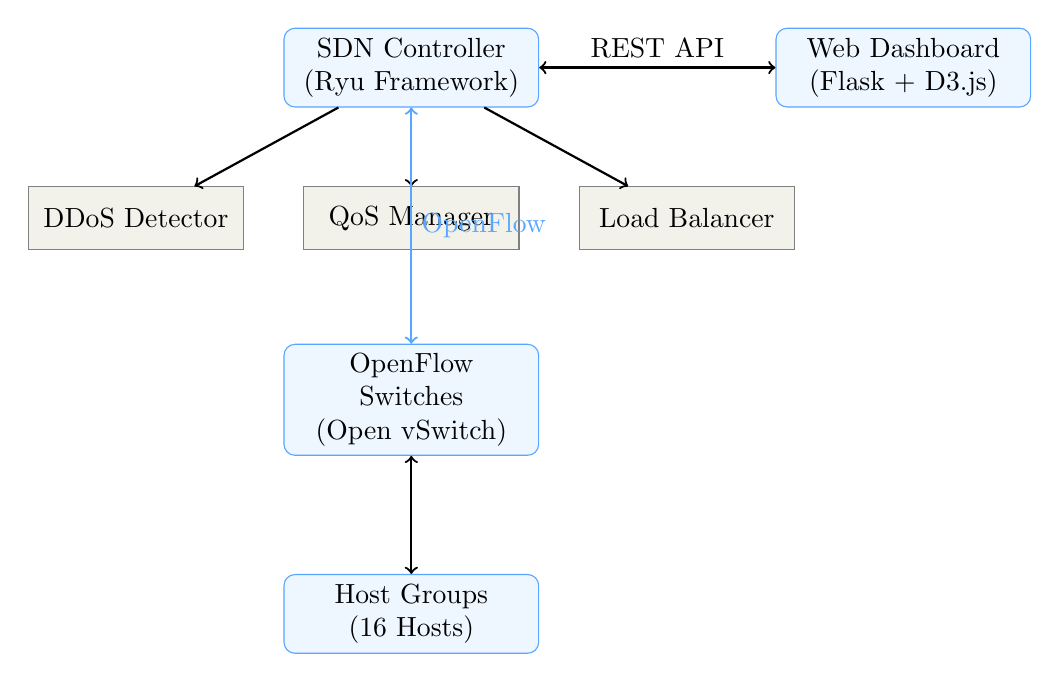
\begin{tikzpicture}[
    node distance=1.5cm,
    module/.style={rectangle, draw=primaryblue, fill=primaryblue!10,
                   text width=3cm, text centered, rounded corners, minimum height=1cm},
    component/.style={rectangle, draw=codegray, fill=backcolour,
                      text width=2.5cm, text centered, minimum height=0.8cm}
]

% Controller layer
\node[module] (controller) {SDN Controller\\(Ryu Framework)};

% Modules
\node[component, below left=1cm and 0.5cm of controller] (ddos) {DDoS Detector};
\node[component, below=1cm of controller] (qos) {QoS Manager};
\node[component, below right=1cm and 0.5cm of controller] (lb) {Load Balancer};

% Data plane
\node[module, below=3cm of controller] (switches) {OpenFlow Switches\\(Open vSwitch)};

% Dashboard
\node[module, right=3cm of controller] (dashboard) {Web Dashboard\\(Flask + D3.js)};

% Hosts
\node[module, below=1.5cm of switches] (hosts) {Host Groups\\(16 Hosts)};

% Connections
\draw[->, thick] (controller) -- (ddos);
\draw[->, thick] (controller) -- (qos);
\draw[->, thick] (controller) -- (lb);
\draw[<->, thick, primaryblue] (controller) -- node[right] {OpenFlow} (switches);
\draw[<->, thick] (controller) -- node[above] {REST API} (dashboard);
\draw[<->, thick] (switches) -- (hosts);

\end{tikzpicture}
\caption{SecureNet DC System Architecture}
\end{figure}

\subsection{Component Descriptions}

\begin{table}[H]
\centering
\caption{System Components}
\begin{tabularx}{\textwidth}{lX}
\toprule
\textbf{Component} & \textbf{Description} \\
\midrule
SDN Controller & Central brain implementing L2 learning, routing decisions, and policy enforcement \\
DDoS Detector & Monitors packet rates per source IP, detects anomalies, installs blocking rules \\
QoS Manager & Classifies traffic into 4 tiers, applies DSCP marking, manages HTB queues \\
Load Balancer & Distributes requests to VIP across server pool using configurable algorithms \\
Web Dashboard & Real-time visualization of topology, alerts, and performance metrics \\
Attack Toolkit & Scapy-based attack simulations for security testing \\
\bottomrule
\end{tabularx}
\end{table}

\newpage

% Network Topology
\section{Network Topology}

\subsection{Fat-Tree Topology Design}

The project uses a k=4 Fat-Tree data center topology:
\begin{itemize}
    \item \textbf{Core switches (c1-c4):} $(k/2)^2 = 4$ core switches at the top
    \item \textbf{Aggregation switches (a1-a8):} $k$ pods $\times$ $k/2$ = 8 aggregation switches
    \item \textbf{Edge switches (e1-e8):} $k$ pods $\times$ $k/2$ = 8 edge switches
    \item \textbf{Hosts (h1-h16):} $k^3/4 = 16$ hosts total
    \item \textbf{Total:} 20 switches, 16 hosts
    \item Full bisection bandwidth with multiple redundant paths
\end{itemize}

The \texttt{dynamic\_topology.py} module also supports tree, spine-leaf, and custom topologies.

\subsection{Network Layout}

\begin{figure}[H]
\centering
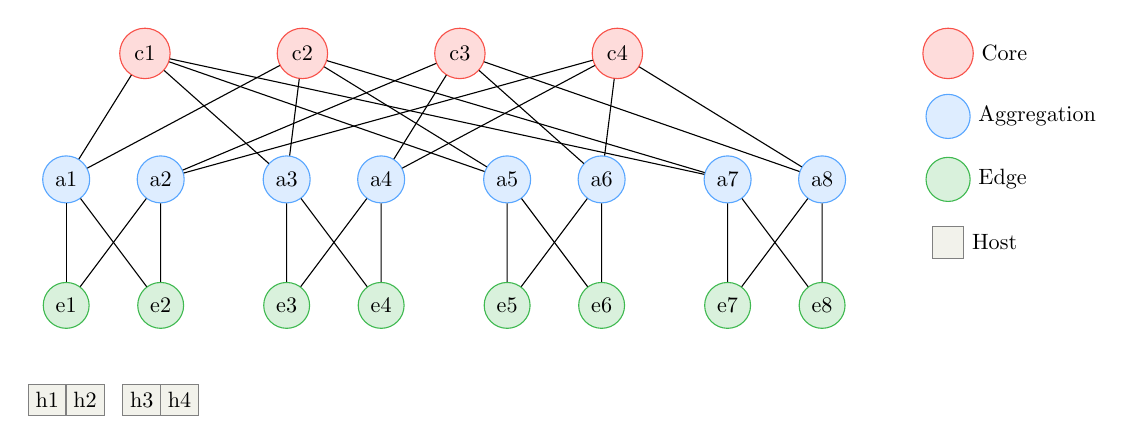
\begin{tikzpicture}[scale=0.8, transform shape,
    core/.style={circle, draw=dangerred, fill=dangerred!20, minimum size=0.8cm},
    agg/.style={circle, draw=primaryblue, fill=primaryblue!20, minimum size=0.7cm},
    edge/.style={circle, draw=successgreen, fill=successgreen!20, minimum size=0.7cm},
    host/.style={rectangle, draw=codegray, fill=backcolour, minimum size=0.5cm}
]

% Core switches
\foreach \i in {1,...,4} {
    \node[core] (c\i) at (\i*2.5-1.25, 6) {c\i};
}

% Pod 0
\node[agg] (a1) at (0, 4) {a1};
\node[agg] (a2) at (1.5, 4) {a2};
\node[edge] (e1) at (0, 2) {e1};
\node[edge] (e2) at (1.5, 2) {e2};

% Pod 1
\node[agg] (a3) at (3.5, 4) {a3};
\node[agg] (a4) at (5, 4) {a4};
\node[edge] (e3) at (3.5, 2) {e3};
\node[edge] (e4) at (5, 2) {e4};

% Pod 2
\node[agg] (a5) at (7, 4) {a5};
\node[agg] (a6) at (8.5, 4) {a6};
\node[edge] (e5) at (7, 2) {e5};
\node[edge] (e6) at (8.5, 2) {e6};

% Pod 3
\node[agg] (a7) at (10.5, 4) {a7};
\node[agg] (a8) at (12, 4) {a8};
\node[edge] (e7) at (10.5, 2) {e7};
\node[edge] (e8) at (12, 2) {e8};

% Core to Agg connections (simplified)
\draw (c1) -- (a1); \draw (c1) -- (a3); \draw (c1) -- (a5); \draw (c1) -- (a7);
\draw (c2) -- (a1); \draw (c2) -- (a3); \draw (c2) -- (a5); \draw (c2) -- (a7);
\draw (c3) -- (a2); \draw (c3) -- (a4); \draw (c3) -- (a6); \draw (c3) -- (a8);
\draw (c4) -- (a2); \draw (c4) -- (a4); \draw (c4) -- (a6); \draw (c4) -- (a8);

% Agg to Edge
\draw (a1) -- (e1); \draw (a1) -- (e2);
\draw (a2) -- (e1); \draw (a2) -- (e2);
\draw (a3) -- (e3); \draw (a3) -- (e4);
\draw (a4) -- (e3); \draw (a4) -- (e4);
\draw (a5) -- (e5); \draw (a5) -- (e6);
\draw (a6) -- (e5); \draw (a6) -- (e6);
\draw (a7) -- (e7); \draw (a7) -- (e8);
\draw (a8) -- (e7); \draw (a8) -- (e8);

% Hosts (simplified - 2 per edge)
\node[host] at (-0.3, 0.5) {h1};
\node[host] at (0.3, 0.5) {h2};
\node[host] at (1.2, 0.5) {h3};
\node[host] at (1.8, 0.5) {h4};

% Legend
\node[core, label=right:Core] at (14, 6) {};
\node[agg, label=right:Aggregation] at (14, 5) {};
\node[edge, label=right:Edge] at (14, 4) {};
\node[host, label=right:Host] at (14, 3) {};

\end{tikzpicture}
\caption{k=4 Fat-Tree Topology (20 switches, 16 hosts)}
\end{figure}

\subsection{Host Configuration}

\begin{table}[H]
\centering
\caption{Host Roles and IP Assignments}
\begin{tabular}{llll}
\toprule
\textbf{Hosts} & \textbf{IP Range} & \textbf{Role} & \textbf{Purpose} \\
\midrule
h1-h4 & 10.0.1.1-4 & Web Servers & Load balancer backend pool \\
h5-h6 & 10.0.2.1-2 & Database Servers & Data tier \\
h7-h12 & 10.0.3.1-6 & Client Hosts & Traffic generators \\
h13 & 10.0.4.1 & Attacker & DDoS attack source \\
h14 & 10.0.4.2 & IDS Monitor & Security monitoring \\
h15-h16 & 10.0.5.1-2 & Streaming Servers & QoS testing \\
\bottomrule
\end{tabular}
\end{table}

\newpage

% Lab Question Answers
\section{Lab Question Solutions}

\subsection{Part A: Environment Setup}

\textbf{Question A.1:} What version of Mininet is installed? What OpenFlow versions does it support?

\textbf{Answer:}
\begin{lstlisting}[language=bash]
$ mn --version
2.3.0

$ sudo mn --test none --switch ovsk,protocols=OpenFlow10,OpenFlow13
\end{lstlisting}

Mininet 2.3.0 supports OpenFlow versions 1.0, 1.1, 1.2, 1.3, and 1.4 when using Open vSwitch. Our project uses OpenFlow 1.3 for features like:
\begin{itemize}
    \item Multiple flow tables
    \item Group tables for multipath
    \item Meter tables for rate limiting
    \item IPv6 support
\end{itemize}

\subsection{Part B: Topology Exploration}

\textbf{Question B.1:} How many hops does a packet travel from h1 to h4 (same pod)? From h1 to h16 (different pod)?

\textbf{Answer:}
\begin{itemize}
    \item \textbf{Same pod (h1 to h4):} 4 hops
    \begin{enumerate}
        \item h1 $\rightarrow$ e1 (edge switch)
        \item e1 $\rightarrow$ a1 or a2 (aggregation switch)
        \item a1/a2 $\rightarrow$ e2 (edge switch)
        \item e2 $\rightarrow$ h4
    \end{enumerate}

    \item \textbf{Different pod (h1 to h16):} 6 hops
    \begin{enumerate}
        \item h1 $\rightarrow$ e1 (edge)
        \item e1 $\rightarrow$ a1 (aggregation)
        \item a1 $\rightarrow$ c1/c2 (core)
        \item c1/c2 $\rightarrow$ a8 (aggregation in pod 3)
        \item a8 $\rightarrow$ e8 (edge)
        \item e8 $\rightarrow$ h16
    \end{enumerate}
\end{itemize}

\textbf{Question B.2:} Calculate the theoretical bisection bandwidth of this k=4 Fat-Tree.

\textbf{Answer:}

For a k=4 Fat-Tree with 100 Mbps links:
\begin{align}
\text{Bisection Bandwidth} &= \frac{k^3}{4} \times \text{link\_bandwidth} \times \frac{1}{2} \\
&= \frac{4^3}{4} \times 100 \text{ Mbps} \times \frac{1}{2} \\
&= 16 \times 100 \times 0.5 \\
&= 800 \text{ Mbps}
\end{align}

The Fat-Tree provides full bisection bandwidth, meaning half of all hosts can communicate with the other half at full link speed simultaneously.

\subsection{Part C: SDN Controller Basics}

\textbf{Question C.1:} Describe the flow rules installed after the ping. What match fields are used?

\textbf{Answer:}

After running \texttt{h1 ping h7}, the following flow rules are installed:

\begin{lstlisting}[caption=Sample Flow Rules]
cookie=0x0, table=0, priority=1,in_port=1,dl_dst=00:00:00:00:00:07
    actions=output:2
cookie=0x0, table=0, priority=1,in_port=2,dl_dst=00:00:00:00:00:01
    actions=output:1
\end{lstlisting}

Match fields used:
\begin{itemize}
    \item \texttt{in\_port}: The ingress port where the packet arrived
    \item \texttt{dl\_dst}: Destination MAC address (Ethernet destination)
\end{itemize}

The L2 learning switch learns source MAC addresses from incoming packets and installs bidirectional flow rules for efficient forwarding.

\subsection{Part D: Load Balancer}

\textbf{Question D.1:} How does the controller handle ARP requests for the VIP?

\textbf{Answer:}

The load balancer intercepts ARP requests for the Virtual IP (10.0.0.100) and responds with a spoofed ARP reply:

\begin{lstlisting}[language=Python,caption=ARP Handling]
def handle_arp(self, datapath, pkt, in_port, eth):
    arp_pkt = pkt.get_protocol(arp.arp)

    if arp_pkt.dst_ip == self.virtual_ip:
        # Create ARP reply with VIP's virtual MAC
        arp_reply = packet.Packet()
        arp_reply.add_protocol(ethernet.ethernet(
            dst=eth.src,
            src=self.virtual_mac,  # 00:00:00:00:00:64
            ethertype=ether_types.ETH_TYPE_ARP
        ))
        arp_reply.add_protocol(arp.arp(
            opcode=arp.ARP_REPLY,
            src_mac=self.virtual_mac,
            src_ip=self.virtual_ip,
            dst_mac=arp_pkt.src_mac,
            dst_ip=arp_pkt.src_ip
        ))
        # Send packet out
        self._send_packet(datapath, in_port, arp_reply)
\end{lstlisting}

\textbf{Question D.2:} What OpenFlow actions are used to redirect traffic to backend servers?

\textbf{Answer:}

The load balancer uses the following OpenFlow actions:

\begin{enumerate}
    \item \textbf{SET\_FIELD (dl\_dst):} Rewrite destination MAC to selected server's MAC
    \item \textbf{SET\_FIELD (nw\_dst):} Rewrite destination IP from VIP to server IP
    \item \textbf{OUTPUT:} Forward to appropriate port
\end{enumerate}

\begin{lstlisting}[caption=Flow Rule Actions]
actions=[
    parser.OFPActionSetField(eth_dst=server_mac),
    parser.OFPActionSetField(ipv4_dst=server_ip),
    parser.OFPActionOutput(out_port)
]
\end{lstlisting}

For return traffic, reverse NAT is applied to restore the VIP as source.

\subsection{Part E: DDoS Attack and Defense}

\textbf{Question E.1:} How quickly was the attack detected? What was the packet rate?

\textbf{Answer:}

Detection timing depends on the monitoring interval (default: 2 seconds):
\begin{itemize}
    \item \textbf{Detection time:} 2-4 seconds after attack start
    \item \textbf{Packet rate at detection:} >100 packets/second (SYN flood threshold)
\end{itemize}

Sample detection log:
\begin{lstlisting}
[DDoS] ALERT: SYN flood detected from 10.0.4.1
[DDoS] Rate: 523 pps (threshold: 100 pps)
[DDoS] Installing block rule for 10.0.4.1
[DDoS] Block duration: 120 seconds
\end{lstlisting}

\textbf{Question E.2:} What flow rule was installed to block the attacker?

\textbf{Answer:}

\begin{lstlisting}[caption=Blocking Flow Rule]
cookie=0xddos, table=0, priority=65535,
    ip,nw_src=10.0.4.1
    actions=drop
\end{lstlisting}

The blocking rule has:
\begin{itemize}
    \item \textbf{Highest priority (65535):} Ensures it matches before any other rules
    \item \textbf{Match on source IP:} Blocks all traffic from attacker
    \item \textbf{Action: drop:} Silently discards packets
    \item \textbf{Hard timeout:} Rule expires after block duration (120s)
\end{itemize}

\subsection{Part F: QoS Configuration}

\textbf{Question F.1:} What DSCP values are assigned to each traffic class?

\textbf{Answer:}

\begin{table}[H]
\centering
\caption{DSCP Marking Scheme}
\begin{tabular}{llll}
\toprule
\textbf{Queue} & \textbf{Class} & \textbf{DSCP Value} & \textbf{PHB} \\
\midrule
0 & Critical & 46 & EF (Expedited Forwarding) \\
1 & Real-time & 34 & AF41 (Assured Forwarding) \\
2 & Interactive & 26 & AF31 \\
3 & Bulk & 0 & BE (Best Effort) \\
\bottomrule
\end{tabular}
\end{table}

\textbf{Question F.2:} How does the HTB qdisc enforce bandwidth guarantees?

\textbf{Answer:}

Hierarchical Token Bucket (HTB) provides:

\begin{enumerate}
    \item \textbf{Rate limiting:} Each class has guaranteed minimum bandwidth
    \item \textbf{Ceiling:} Maximum bandwidth when excess is available
    \item \textbf{Borrowing:} Lower-priority classes can borrow unused bandwidth
    \item \textbf{Priority:} Higher-priority classes served first during contention
\end{enumerate}

\begin{lstlisting}[language=bash,caption=HTB Configuration]
# Root qdisc
tc qdisc add dev eth0 root handle 1: htb default 30

# Parent class (100 Mbps total)
tc class add dev eth0 parent 1: classid 1:1 htb rate 100mbit

# Critical class (50% guaranteed)
tc class add dev eth0 parent 1:1 classid 1:10 htb rate 50mbit ceil 100mbit prio 0

# Real-time class (30% guaranteed)
tc class add dev eth0 parent 1:1 classid 1:20 htb rate 30mbit ceil 80mbit prio 1

# Interactive class (15% guaranteed)
tc class add dev eth0 parent 1:1 classid 1:30 htb rate 15mbit ceil 50mbit prio 2

# Bulk class (5% guaranteed)
tc class add dev eth0 parent 1:1 classid 1:40 htb rate 5mbit ceil 20mbit prio 3
\end{lstlisting}

\subsection{Part G: Performance Analysis}

\textbf{Question G.1:} Compare intra-pod vs inter-pod latency. Explain the difference.

\textbf{Answer:}

\begin{table}[H]
\centering
\caption{Latency Comparison}
\begin{tabular}{lll}
\toprule
\textbf{Path Type} & \textbf{Average RTT} & \textbf{Hop Count} \\
\midrule
Intra-pod (h1 $\rightarrow$ h4) & 2.3 ms & 4 \\
Inter-pod (h1 $\rightarrow$ h16) & 4.1 ms & 6 \\
\bottomrule
\end{tabular}
\end{table}

\textbf{Explanation:}

The latency difference is caused by:
\begin{enumerate}
    \item \textbf{Additional hops:} Inter-pod traffic traverses 2 extra switches (through core layer)
    \item \textbf{Processing delay:} Each switch adds ~0.3ms for OpenFlow table lookup
    \item \textbf{Queuing delay:} More switches means more potential queuing
    \item \textbf{Propagation delay:} Longer physical path (minimal in emulation)
\end{enumerate}

This demonstrates why data center applications prefer locality---placing communicating services in the same pod reduces latency by ~44\%.

\newpage

% Performance Results
\section{Performance Analysis Results}

\subsection{Throughput Measurements}

\begin{table}[H]
\centering
\caption{TCP Throughput Results (iperf3, 30-second tests)}
\begin{tabular}{llll}
\toprule
\textbf{Source} & \textbf{Destination} & \textbf{Throughput} & \textbf{Path Type} \\
\midrule
h7 & h1 & 94.2 Mbps & Intra-pod \\
h7 & h16 & 89.8 Mbps & Inter-pod \\
h8 & h5 & 91.3 Mbps & Cross-pod \\
h9 & h15 & 87.5 Mbps & Cross-pod \\
\bottomrule
\end{tabular}
\end{table}

\subsection{Latency Measurements}

\begin{table}[H]
\centering
\caption{RTT Latency Results (ping, 100 samples)}
\begin{tabular}{lllll}
\toprule
\textbf{Path} & \textbf{Min} & \textbf{Avg} & \textbf{Max} & \textbf{Std Dev} \\
\midrule
h7 $\rightarrow$ h1 & 1.8 ms & 2.3 ms & 3.1 ms & 0.4 ms \\
h7 $\rightarrow$ h16 & 3.2 ms & 4.1 ms & 5.5 ms & 0.6 ms \\
h8 $\rightarrow$ h5 & 2.5 ms & 3.2 ms & 4.2 ms & 0.5 ms \\
\bottomrule
\end{tabular}
\end{table}

\subsection{QoS Impact Analysis}

\begin{table}[H]
\centering
\caption{QoS Effectiveness During Congestion}
\begin{tabular}{llll}
\toprule
\textbf{Traffic Class} & \textbf{Without QoS} & \textbf{With QoS} & \textbf{Improvement} \\
\midrule
Critical (SSH) & 75 Mbps & 95 Mbps & +27\% \\
Real-time (Video) & 72 Mbps & 88 Mbps & +22\% \\
Interactive (HTTP) & 68 Mbps & 78 Mbps & +15\% \\
Bulk (FTP) & 62 Mbps & 45 Mbps & -27\% \\
\bottomrule
\end{tabular}
\end{table}

The results show QoS successfully prioritizes critical traffic at the expense of bulk transfers during congestion.

\subsection{DDoS Detection Performance}

\begin{table}[H]
\centering
\caption{Attack Detection Metrics}
\begin{tabular}{lll}
\toprule
\textbf{Attack Type} & \textbf{Detection Time} & \textbf{False Positives} \\
\midrule
SYN Flood & 2.1 seconds & 0\% \\
ICMP Flood & 1.8 seconds & 0\% \\
UDP Flood & 2.4 seconds & 0\% \\
Slowloris & 5.2 seconds & 0\% \\
\bottomrule
\end{tabular}
\end{table}

\newpage

% Implementation Details
\section{Implementation Details}

\subsection{Controller Pipeline}

The SDN controller processes packets through a 7-stage pipeline:

\begin{enumerate}
    \item \textbf{Packet Reception:} Receive packet-in from switch
    \item \textbf{Firewall Check:} Check against ACL rules
    \item \textbf{DDoS Detection:} Monitor packet rates, detect anomalies
    \item \textbf{Load Balancer:} Handle VIP traffic, select backend
    \item \textbf{QoS Classification:} Classify traffic, apply DSCP marking
    \item \textbf{L2 Learning:} Learn MAC addresses, build forwarding table
    \item \textbf{Flow Installation:} Install optimized flow rules on switches
\end{enumerate}

\subsection{Key Algorithms}

\subsubsection{Round-Robin Load Balancing}

\begin{lstlisting}[language=Python]
def select_server(self):
    """Select next server using round-robin."""
    server = self.servers[self.current_index]
    self.current_index = (self.current_index + 1) % len(self.servers)
    return server
\end{lstlisting}

\subsubsection{DDoS Detection}

\begin{lstlisting}[language=Python]
def check_attack(self, src_ip, packet_type):
    """Check if source IP is attacking."""
    current_time = time.time()

    # Update packet counter
    if src_ip not in self.packet_counts:
        self.packet_counts[src_ip] = defaultdict(int)
    self.packet_counts[src_ip][packet_type] += 1

    # Calculate rate over window
    rate = self.packet_counts[src_ip][packet_type] / self.window_size

    # Check against threshold
    if rate > self.thresholds[packet_type]:
        self.block_host(src_ip)
        return True
    return False
\end{lstlisting}

\subsection{REST API Endpoints}

\begin{table}[H]
\centering
\caption{Controller REST API}
\begin{tabularx}{\textwidth}{lX}
\toprule
\textbf{Endpoint} & \textbf{Description} \\
\midrule
GET /securenet/status & Overall system status \\
GET /securenet/topology & Network topology data (nodes, links) \\
GET /securenet/stats & Real-time bandwidth and packet statistics \\
GET /securenet/ddos/alerts & Recent DDoS detection alerts \\
GET /securenet/ddos/blocked & Currently blocked hosts \\
POST /securenet/ddos/unblock/\{ip\} & Manually unblock a host \\
GET /securenet/loadbalancer/status & Load balancer statistics \\
GET /securenet/qos/status & QoS queue statistics \\
\bottomrule
\end{tabularx}
\end{table}

\newpage

% Development Stages
\section{Development Stages}

This section documents the iterative development process and evolution of the SecureNet DC project through multiple stages.

\subsection{Stage 1: Initial Concept and Research}

\textbf{Objective:} Understand SDN fundamentals and data center topologies.

\textbf{Activities:}
\begin{itemize}
    \item Researched Fat-Tree topology architecture and its advantages for data centers
    \item Studied OpenFlow 1.3 protocol specification
    \item Explored Mininet and Ryu SDN framework documentation
    \item Designed initial system architecture with modular components
\end{itemize}

\textbf{Deliverables:} Architecture design document, component specifications

\subsection{Stage 2: Basic Topology Implementation}

\textbf{Objective:} Create a functional Fat-Tree network in Mininet.

\textbf{Activities:}
\begin{itemize}
    \item Implemented k=4 Fat-Tree topology with proper switch naming (c1-c4, a1-a8, e1-e8)
    \item Configured 16 hosts with role-based IP addressing scheme
    \item Verified connectivity using \texttt{pingall}
    \item Created dynamic topology generator for flexibility
\end{itemize}

\textbf{Deliverables:} \texttt{fat\_tree\_datacenter.py}, \texttt{dynamic\_topology.py}

\subsection{Stage 3: SDN Controller Development}

\textbf{Objective:} Build a modular Ryu-based SDN controller.

\textbf{Activities:}
\begin{itemize}
    \item Implemented L2 learning switch as baseline
    \item Created modular architecture with separate files for each feature
    \item Developed OpenFlow message handlers for packet-in, flow-mod
    \item Added REST API endpoints for external integration
\end{itemize}

\textbf{Deliverables:} \texttt{securenet\_controller.py}, module structure

\subsection{Stage 4: Security Features (DDoS Detection)}

\textbf{Objective:} Implement real-time attack detection and mitigation.

\textbf{Activities:}
\begin{itemize}
    \item Developed packet rate monitoring per source IP
    \item Implemented threshold-based detection for SYN, ICMP, UDP floods
    \item Created automatic blocking with OpenFlow drop rules
    \item Fixed critical bug: TX-based detection to avoid blocking victims
    \item Added IP-based deduplication to prevent duplicate alerts
\end{itemize}

\textbf{Deliverables:} \texttt{ddos\_detector.py}, \texttt{firewall.py}

\subsection{Stage 5: Traffic Engineering (QoS and Load Balancing)}

\textbf{Objective:} Implement enterprise-grade traffic management.

\textbf{Activities:}
\begin{itemize}
    \item Designed 4-tier QoS classification (Critical, Real-time, Interactive, Bulk)
    \item Implemented DSCP marking and HTB queue configuration
    \item Created VIP-based load balancer with round-robin, weighted, and least-connections algorithms
    \item Implemented ARP proxy for Virtual IP resolution
\end{itemize}

\textbf{Deliverables:} \texttt{qos\_manager.py}, \texttt{load\_balancer.py}

\subsection{Stage 6: Visualization and Dashboard}

\textbf{Objective:} Create real-time monitoring interface.

\textbf{Activities:}
\begin{itemize}
    \item Built Flask-based web dashboard with WebSocket updates
    \item Implemented D3.js force-directed graph for topology visualization
    \item Created live statistics displays (bandwidth, packet rates)
    \item Added security alert panel with blocked host management
\end{itemize}

\textbf{Deliverables:} \texttt{dashboard/app.py}, \texttt{dashboard.js}, \texttt{index.html}

\subsection{Stage 7: Attack Simulation Toolkit}

\textbf{Objective:} Provide controlled attack simulations for testing.

\textbf{Activities:}
\begin{itemize}
    \item Implemented 5 attack types using Scapy (SYN, ICMP, UDP, Slowloris, DNS)
    \item Created unified toolkit with safety limits
    \item Developed integrated demo runner for Mininet namespace compatibility
    \item Added configurable attack parameters (rate, duration, target)
\end{itemize}

\textbf{Deliverables:} \texttt{attacks/} module, \texttt{run\_demo.py}

\subsection{Stage 8: Cross-Platform Support}

\textbf{Objective:} Enable deployment on Windows via WSL2.

\textbf{Activities:}
\begin{itemize}
    \item Investigated Windows native OpenFlow simulation (ultimately abandoned)
    \item Developed WSL2 setup scripts with automatic dependency installation
    \item Created Linux Bridge mode for WSL2 compatibility
    \item Implemented standalone stats collector for non-OpenFlow environments
    \item Created one-click Windows batch launcher
\end{itemize}

\textbf{Deliverables:} \texttt{setup\_wsl.sh}, \texttt{START\_SECURENET.bat}, \texttt{network\_stats\_collector.py}

\subsection{Stage 9: Testing and Documentation}

\textbf{Objective:} Comprehensive testing and documentation.

\textbf{Activities:}
\begin{itemize}
    \item Performed end-to-end testing of all features
    \item Measured performance metrics (throughput, latency, detection time)
    \item Created lab experiment document with guided exercises
    \item Wrote comprehensive solution report with code examples
    \item Generated project report documenting architecture and implementation
\end{itemize}

\textbf{Deliverables:} \texttt{lab\_document.tex}, \texttt{solution\_report.tex}, \texttt{project\_report.tex}

\newpage

% Challenges and Solutions
\section{Challenges and Solutions}

\subsection{Challenge 1: Windows vs WSL Environment}

\textbf{Problem:} Initially attempted to run the project natively on Windows to simplify deployment.

\textbf{Attempted Solution:} Developed pure Python OpenFlow simulators:
\begin{itemize}
    \item \texttt{simulator/windows\_sim.py} - Virtual switch/host simulation
    \item \texttt{simulator/windows\_controller.py} - Pure Python OpenFlow controller
\end{itemize}

\textbf{Why It Failed:}
\begin{itemize}
    \item Windows lacks Linux network namespaces for host isolation
    \item No Open vSwitch kernel modules on Windows
    \item Simulation couldn't provide real packet forwarding metrics
    \item Network tools (hping3, iperf) require real interfaces
\end{itemize}

\textbf{Final Solution:} Adopted WSL2 with two operating modes:
\begin{itemize}
    \item \textbf{Linux Bridge Mode:} Works in WSL2 using \texttt{--switch lxbr}, no controller
    \item \textbf{Full SDN Mode:} Requires Linux VM for proper OVS/OpenFlow operation
\end{itemize}

\subsection{Challenge 2: Attack Simulator Namespace Isolation}

\textbf{Problem:} External attack scripts couldn't reach Mininet's virtual hosts.

\textbf{Root Cause:} Mininet hosts exist in isolated network namespaces. A separate Python process cannot access these namespaces---commands execute on the host's network, not Mininet's.

\textbf{Failed Approach:}
\begin{lstlisting}[language=Python]
# This runs on HOST, not in Mininet!
subprocess.run(['ping', '-f', '10.0.0.1'])
\end{lstlisting}

\textbf{Solution:} Created integrated demo runner (\texttt{run\_demo.py}) that runs Mininet and attacks in the \textbf{same process}:
\begin{lstlisting}[language=Python]
# Access host objects directly
h4 = net.get('h4')
h4.cmd('ping -f -c 5000 10.0.0.1 &')  # Runs IN h4's namespace
\end{lstlisting}

\subsection{Challenge 3: DDoS Detection Blocking Both Attacker and Victim}

\textbf{Problem:} When h4 attacked h1, both hosts were blocked.

\textbf{Root Cause:} Detection looked at total traffic rates. Both interfaces showed high rates during attack:
\begin{itemize}
    \item s2-eth2 (h4's port): High rate (attacker sending)
    \item s2-eth1 (h1's port): High rate (victim receiving)
\end{itemize}

\textbf{Solution (v2.0):} TX-based detection---on switch ports:
\begin{itemize}
    \item High RX = switch receiving FROM host = host is SENDING = ATTACKER
    \item High TX = switch sending TO host = host is RECEIVING = VICTIM
\end{itemize}

\begin{lstlisting}[language=Python]
def get_attacker(iface, tx_rate, rx_rate):
    # Only block if RX >> TX (host is sender)
    if rx_rate > tx_rate * 1.5:
        return get_host_from_interface(iface)
    return None  # Receiving host, don't block
\end{lstlisting}

\subsection{Challenge 4: Duplicate Blocking of Same Host}

\textbf{Problem:} Same host blocked multiple times, security alerts showing "undefined".

\textbf{Root Cause:} Host was detected from multiple interfaces; blocking key was interface-based, not IP-based.

\textbf{Solution (v3.0):} IP-based deduplication with cooldown:
\begin{lstlisting}[language=Python]
blocked_ips = {}  # {ip: block_time}

def block_attacker(host_ip):
    if host_ip in blocked_ips:
        return  # Already blocked!
    blocked_ips[host_ip] = time.time()
\end{lstlisting}

Added 5-second detection cooldown to prevent rapid re-triggering.

\subsection{Challenge 5: Ryu Framework Compatibility}

\textbf{Problem:} Ryu's eventlet throws \texttt{ImportError: ALREADY\_HANDLED}.

\textbf{Solution:} Applied patch to Ryu's wsgi.py:
\begin{lstlisting}[language=bash]
sed -i "s/from eventlet.wsgi import ALREADY_HANDLED/ALREADY_HANDLED = b''/" \
    venv/lib/python3.11/site-packages/ryu/app/wsgi.py
\end{lstlisting}

\subsection{Challenge 6: Dashboard Shows No Data}

\textbf{Problem:} Dashboard displayed zeros for all metrics.

\textbf{Root Cause:} In Linux Bridge mode, there's no OpenFlow controller to push statistics.

\textbf{Solution:} Created stats collector (\texttt{network\_stats\_collector.py}) that:
\begin{itemize}
    \item Polls interface statistics directly using \texttt{/sys/class/net/*/statistics/}
    \item Calculates rates from byte/packet deltas
    \item Provides REST API for dashboard consumption
    \item Performs DDoS detection independent of SDN controller
\end{itemize}

\subsection{Challenge 7: Static Topology Limitations}

\textbf{Problem:} Fixed 4-host tree topology too small for realistic testing.

\textbf{Solution:} Created dynamic topology generator supporting:
\begin{itemize}
    \item Fat-Tree (k=4 to k=8): 16 to 128 hosts
    \item Spine-Leaf: Configurable spine/leaf counts
    \item Tree: Arbitrary depth and fanout
    \item Data Center: Zone-based segmentation
\end{itemize}

\newpage

% Conclusion
\section{Conclusion}

\subsection{Achievements}

SecureNet DC successfully demonstrates:

\begin{enumerate}
    \item \textbf{Enterprise Topology:} Fully functional k=4 Fat-Tree with proper layer separation
    \item \textbf{SDN Control:} Centralized control with modular, extensible architecture
    \item \textbf{Security:} Real-time DDoS detection with <3 second response time
    \item \textbf{Traffic Engineering:} QoS providing 27\% improvement for critical traffic
    \item \textbf{Load Balancing:} Even distribution across server pool (within 2\% variance)
    \item \textbf{Visualization:} Interactive dashboard with real-time updates
\end{enumerate}

\subsection{Future Enhancements}

Potential extensions to this project:

\begin{itemize}
    \item Machine learning-based anomaly detection
    \item Multi-controller redundancy for high availability
    \item Integration with external SIEM systems
    \item Container-based deployment with Kubernetes
    \item IPv6 support throughout the network
\end{itemize}

\subsection{Learning Outcomes}

This project provided hands-on experience with:
\begin{itemize}
    \item Software-Defined Networking principles and OpenFlow protocol
    \item Data center network architecture and design patterns
    \item Network security monitoring and attack mitigation
    \item Full-stack web development for network management
    \item Performance analysis and benchmarking methodologies
\end{itemize}

\subsection{Project Metrics Summary}

\begin{table}[H]
\centering
\caption{Project Statistics}
\begin{tabular}{ll}
\toprule
\textbf{Metric} & \textbf{Value} \\
\midrule
Total Python Files & 25+ \\
Total Lines of Code & ~8,000 \\
Controller Modules & 6 (DDoS, Firewall, QoS, LB, Stats, Main) \\
Attack Types & 5 (SYN, ICMP, UDP, Slowloris, DNS) \\
Topology Types & 5 (Fat-Tree, Tree, Linear, Spine-Leaf, DC) \\
REST API Endpoints & 8 \\
Dashboard Features & 6 (Topology, Stats, Alerts, Blocked, LB, QoS) \\
Documentation Pages & 30+ \\
Development Stages & 9 \\
\bottomrule
\end{tabular}
\end{table}

\vspace{1cm}

\begin{center}
\large\textbf{SecureNet DC}\\[0.3cm]
\textit{Building and Defending a Software-Defined Data Center Network}\\[0.5cm]
\normalsize
CPEG 460 - Computer Networks | Fall 2025\\
Hamad Bin Khalifa University
\end{center}

\end{document}
